\documentclass[a4paper,13.5pt]{extarticle}
\usepackage{geometry}
\usepackage[utf8]{inputenc}
\usepackage{amsmath,amssymb,graphicx,mathtools, nccmath, bigints}
\usepackage{caption,subcaption}
\usepackage{multirow}
\usepackage{float}
\usepackage{lipsum}
\usepackage{hyperref}
\usepackage{enumitem}
\usepackage[nodisplayskipstretch]{setspace}
\usepackage{booktabs}
\usepackage{mathtools}
\usepackage{etoolbox}
\usepackage{xcolor}
\usepackage[capitalize]{cleveref}
\usepackage{blindtext}
\usepackage{eso-pic,rotating,graphicx}
\usepackage{microtype}
\usepackage{scalerel}


\newcommand{\argmax}{\operatornamewithlimits{argmax}}
\def\am{$\theta_{\scaleto{\text{AM}}{2pt}}$}
\title{WFST enabled Maximum Conditional Log-Likelihood~(MCLL) Training}
\author{Tina Raissi}


\begin{document}
	
	\maketitle
	
	\section{Training Criterion}
	For an acoustic feature sequence $X = x_1^T$ and a word sequence $W = w_1^N$, of length $T$ and $N$, respectively, define the output sequence $a_1^S$ corresponding to $W$.\  This can be phonemes, wordpieces, or characters.\ Moreover, consider $y_1^T$ to be the blank augmented sequence of frame labels. There is a mapping function that reduces the alignment sequence to the output sequence by eliminating blanks and label loops.
	
	For a set of parameters $\theta$, the statistical formulation of automatic speech recognition task based on conditional likelihood is defined as:
	
	
	\begin{align}
		\label{CL}
		\mathcal{F_{\text{CL}}}(\theta) & = \frac{1}{R}\sum_{r=1}^R p_{_\theta}(a_1^{S_r} | X^r)\\
		& = \frac{1}{R}\sum_{r=1}^R \sum_{y_1^{T^r}:a_1^{S^r}} \prod_ t  p_{\theta}(y_t | X^r)
	\end{align}

We now pass to log and drop the constant value and consider one pair of $(a_1^S , X)$. For simplicity, we take a context-independent, 1-gram with context 0 model.

	\begin{align}
	\label{CLL}
	\mathcal{F_{\text{CLL}}}(\theta) & =\sum_{t=1}^T \sum_{y_1^{T}:a_1^{S}}  \log p_{\theta}(y_t | X)
\end{align}


Define the quantity $q_t$ as the state marginal or occupancy as:

\begin{align}
	q_t(y|X,\theta) = \frac{ \sum_{\substack{y_1^{T}:a_1^{S} \\ y_t=y} }\prod_{\tau=1}^T  p_{\theta} (y_{\tau} | X)}{\sum_{\substack{y_1^{T}:a_1^{S}} } p_{\theta} (y_1^T | X)}
\end{align}

We can carry out the derivative as follows:


	\begin{align*}
		\frac{\partial}{\partial \theta} \mathcal{F_{\text{CLL}}}(\theta) = \sum_{t}\sum_{y}{q_t(y|X,\theta)}\cdot \frac{\partial}{\partial \theta}  \log p_t(y_t|X,\theta)
\end{align*}%

For a model with context one the probability $p(y_t|X)$ at step $t$ would be substituted by $p(y_t|a_{s_{t-1}}, X)$, as an example.

	
	
	
	
	
	
	
	\section{WFST/Graph Representation}
	
	For decoding or sequence discriminative training we generally need to consider the set of all possible word sequences called also as the hypothesis space. This can be done by taking an N-best list of the most likely hypotheses or to use lattices, called sometimes also as graphs or Lattices.
	
	A transducer $\mathcal{L}$ is an a-cyclic graph where nodes represent the time steps and edges represent the words. Each arc can be augmented with weights. Each path $\pi$ through $\mathcal{L}$  consists of a sequence of edges $e_1^N$ corresponding to a word sequence of length $N$. \ The edges carry the product of the acoustic and language model.
	
	\begin{align}
		\label{probpath}
		p(e_1^N, X) = \prod_{n=1}^N w[e_n]
	\end{align}
	
	The probability of a certain word within the sequence is equal to the sum over probability of all transducer paths $\pi(\mathcal{L})$ going through that specific edge:
	
	\begin{align}
		\label{probedge}
		p(e | X) = \sum_{\substack{e_1^N \in \pi(\mathcal{L})\\ \exists n: e_n=e}}p(e_1^N | X)
	\end{align}
	
	The sum over all paths is generally carried out via forward-backward algorithm. Denote forward and backward scores accumulated at a certain transducer node $s$ by $\phi(s)$ and $\psi(s)$, respectively. For partial edge sequences $e_1^k$ and  $e_h^N$ reaching the edge $e$ in forward and backward paths we have
	
	\begin{align}
		\label{fwdbkwd}
		\mathbf{fb}(e, X)  = \sum_{\substack{e_1^k: \\ n[e_k] = p[e]}}\prod_{m=1}^k w[e_m] \cdot w[e] \cdot  \sum_{\substack{e_h^N: \\ p[e_h] = n[e]}}\prod_{n=h}^N w[e_n] 
	\end{align}
	
	Following \cref{fwdbkwd}, we can calculate the prior as $\phi(F) = p(X)$. Consequently, it is possible to calculate the arc posterior as $\mathbf{fb}(e | X) = \frac{	\mathbf{fb}(e, X)}{ p(X)}$.
	
	
	\begin{figure}[t]
		\centering
		\caption*{Definition of different semirings relevant for training and decoding in ASR.(Source: \cite{hoffmeister2011wfst})}
		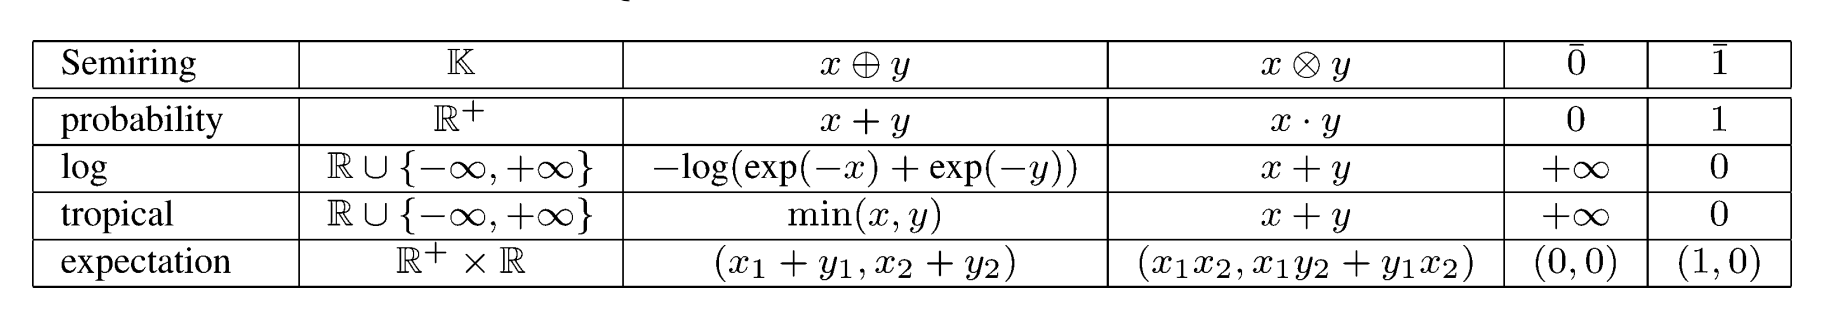
\includegraphics[width=1.\linewidth]{figures/semirings}	
	\end{figure}
	
	
	
	\bibliographystyle{IEEEtran}
	\bibliography{mybib}
	
	
	
	
	
	
	
	
	
	
\end{document}
